
\subsection{Définitions}

\begin{frame}{Définitions (1/2) -- Déplacement égocentrique}
    \begin{columns}
        \begin{column}{0.49\textwidth}
            \begin{block}{Repère égocentrique}
                Projection du repère du buste
            \end{block}
            \begin{block}{Pose}
                Position + orientation $\in \mathbb{R}^2 \times ]-\pi,\pi]$
            \end{block}
            \begin{block}{Pied de support}
                Pied en contact avec le sol
            \end{block}
            \begin{block}{Déplacement égocentrique}
                Variation de la pose du repère égocentrique
                entre deux changements de pied de support
                $
                \Delta \bm{p} =
                \begin{bmatrix}
                    \Delta x \\ \Delta y \\ \Delta \theta 
                \end{bmatrix}
                \in \mathbb{R}^3
                $
            \end{block}
        \end{column}
        \begin{column}{0.49\textwidth}
            \centering
            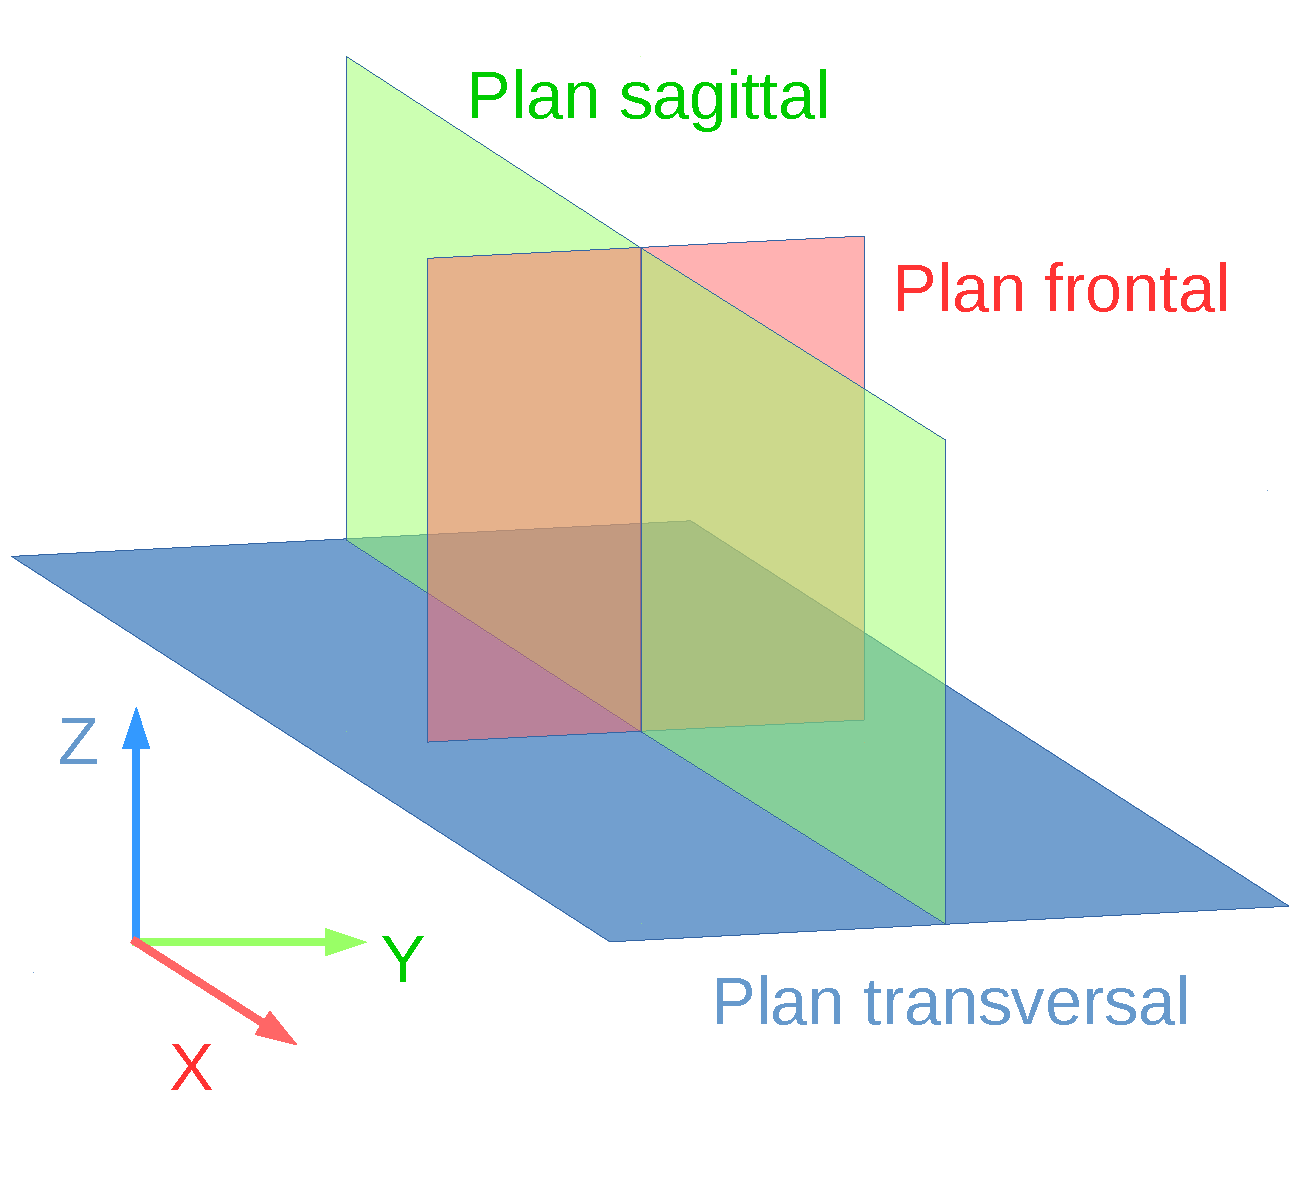
\includegraphics[type=pdf,ext=.pdf,read=.pdf,width=0.6\linewidth]{../schema/planes}
            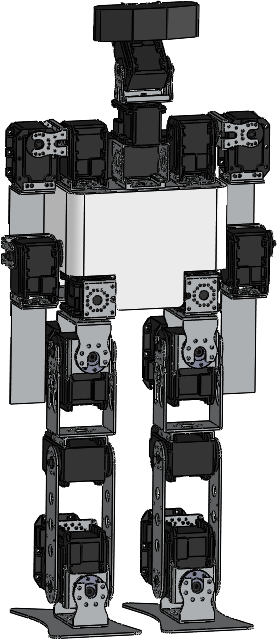
\includegraphics[width=0.25\linewidth]{../media/sigmaban_cao2.png}
            \newline
            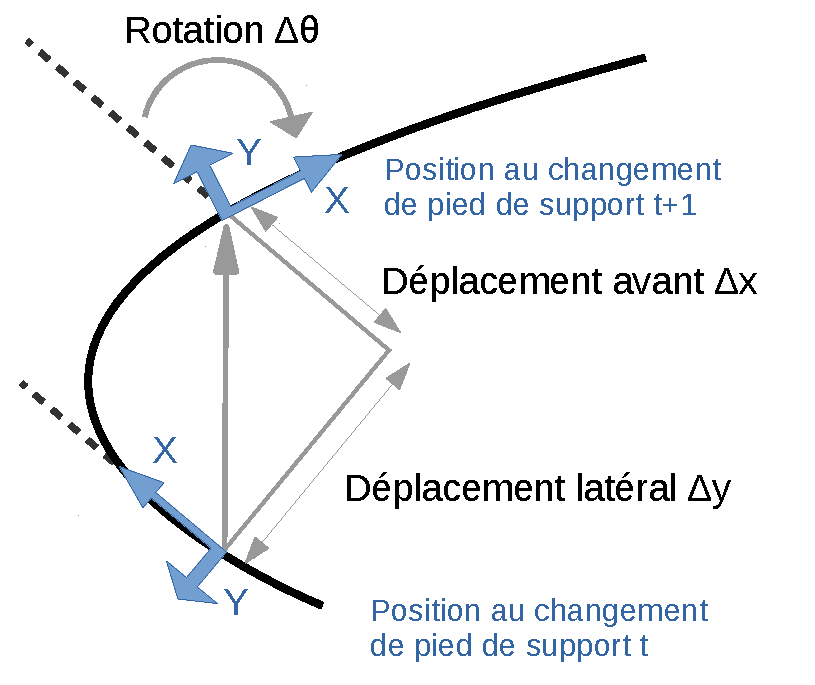
\includegraphics[type=pdf,ext=.pdf,read=.pdf,width=0.9\linewidth]{../schema/footstep}
        \end{column}
    \end{columns}
\end{frame}

\begin{frame}{Définitions (2/2) -- Odométrie proprioceptive et prédictive}
    \begin{block}{Odométrie proprioceptive}
        \begin{columns}
            \begin{column}{0.4\textwidth}
                Capteurs proprioceptifs
                (encodeurs, IMU, pression)
            \end{column}
            \begin{column}{0.2\textwidth}
                $\longmapsto$
            \end{column}
            \begin{column}{0.3\textwidth}
                Déplacements égocentriques
            \end{column}
        \end{columns}
    \end{block}
    \begin{block}{Odométrie prédictive (modèle de déplacement)}
        \begin{columns}
            \begin{column}{0.4\textwidth}
                Ordres de la marche
            \end{column}
            \begin{column}{0.2\textwidth}
                $\longmapsto$
            \end{column}
            \begin{column}{0.3\textwidth}
                Déplacements égocentriques
            \end{column}
        \end{columns}
    \end{block}
    \vspace{2.0em}
    \begin{itemize}
        \item Pas de caméra
        \item Précision odométrie proprioceptive > prédictive
        \item Apprentissage avec les mêmes données
        \item Intégration $\Rightarrow$ trajectoire
    \end{itemize}
\end{frame}

\subsection{Enjeux}

\begin{frame}{Applications pour la RoboCup}
    \begin{columns}
        \begin{column}{0.49\linewidth}
            Odométrie proprioceptive :
            \begin{itemize}
                \item Localisation
                \item Asservissement du déplacement
                \item Suivi de la balle
            \end{itemize}
        \end{column}
        \begin{column}{0.49\linewidth}
            Odométrie prédictive :
            \begin{itemize}
                \item Simulation du déplacement
                \item Tests comportements haut niveau
                \item Plannification de trajectoire
            \end{itemize}
        \end{column}
    \end{columns}
    \vspace{0.2cm}
    \centering
    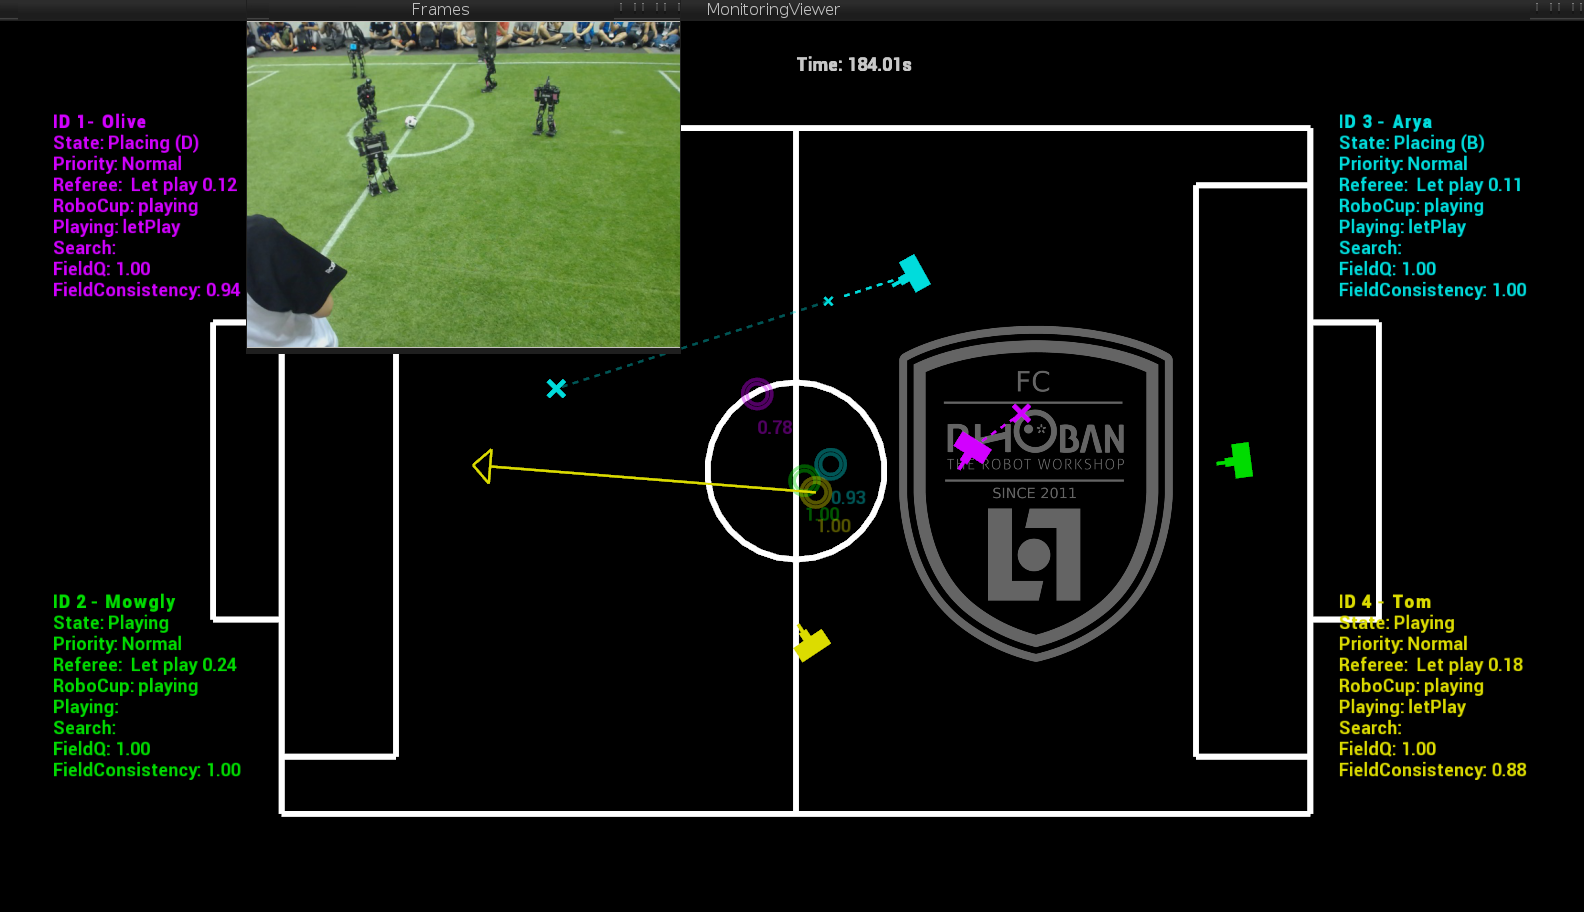
\includegraphics[width=0.85\linewidth]{../media/monitoring.png}
\end{frame}

